\newpage

\subsection{Duplicating elements via drag-and-drop}

Sometimes you'll have an element (or many) that are nearly identical, and life would be \emph{so} much easier if you could copy and paste an existing one
already. Suppose you want a copy of a \texttt{this} element, so you press \texttt{Ctrl + C}, followed by \texttt{Ctrl + V}. An error dialogue preventing the
action will immediately raise, stating that the ``\ldots diagram already contains an instance of the element you are trying to paste.'' EA can only support
unique objects, so you'll need to use the following process.

\begin{itemize}

\item[$\blacktriangleright$] In either a diagram or in the project browser, hold \texttt{Ctrl}, then drag the element you wish to duplicate. A
confirmation-style dialogue will appear (Fig.~\ref{ea:dupWindow}), and a properties window will follow. You must assign a unique name to the new element, or
else you'll receive an error when you try to export the project later.

\vspace{0.5cm}

\begin{figure}[htbp]
\begin{center}
  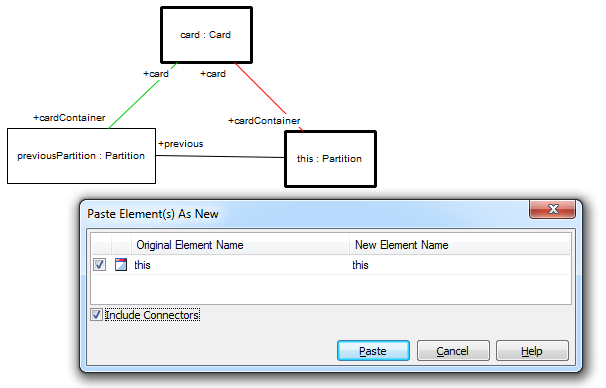
\includegraphics[width=0.95\textwidth]{ea_duplicatingElements}
  \caption{Copying elements}  
  \label{ea:dupWindow}
\end{center}
\end{figure}

\end{itemize}
